\documentclass[tikz,border=4pt]{standalone}
\usepackage{pgfplots}\usepgfplotslibrary{groupplots}
\pgfplotsset{compat=1.18}
\definecolor{tramU}{HTML}{365FB3}\definecolor{tramDos}{HTML}{0F766E}\definecolor{punt}{HTML}{B91C1C}
\begin{document}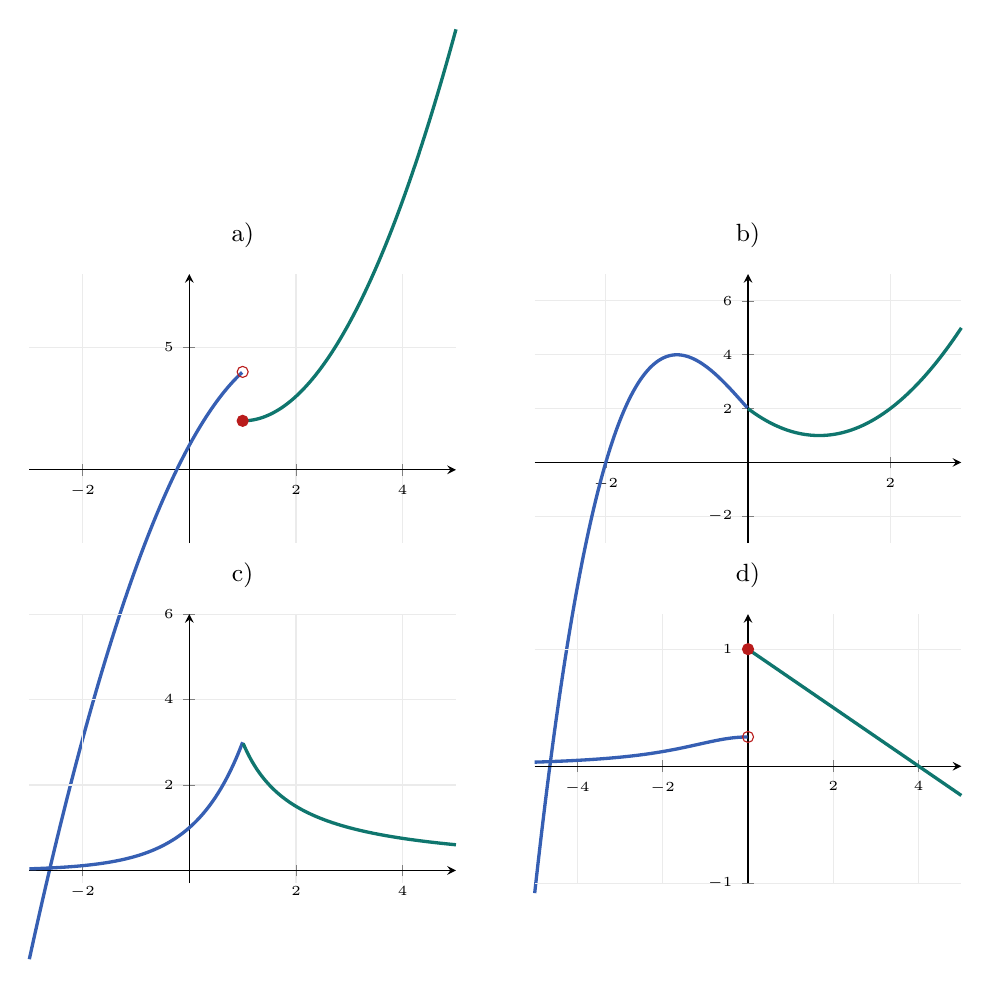
\begin{tikzpicture}
\begin{groupplot}[group style={group size=2 by 2,horizontal sep=1cm,vertical sep=0.9cm},
 width=7cm,height=5cm,axis lines=middle,grid=major,grid style={black!8},tick label style={font=\tiny},title style={font=\small},samples=120,clip=false]
\nextgroupplot[title={a)},xmin=-3,xmax=5,ymin=-3,ymax=8]\addplot[tramU,very thick,domain=-3:.99]{-x^2+4*x+1};\addplot[tramDos,very thick,domain=1:5]{x^2-2*x+3};\addplot[only marks,mark=o,punt,fill=white] coordinates {(1,4)};\addplot[only marks,mark=*,punt] coordinates {(1,2)};
\nextgroupplot[title={b)},xmin=-3,xmax=3,ymin=-3,ymax=7]\addplot[tramU,very thick,domain=-3:-.01]{x^3-3*x+2};\addplot[tramDos,very thick,domain=0:3]{(x-1)^2+1};
\nextgroupplot[title={c)},xmin=-3,xmax=5,ymin=-.3,ymax=6]\addplot[tramU,very thick,domain=-3:1]{3^x};\addplot[tramDos,very thick,domain=1.01:5]{3/x};
\nextgroupplot[title={d)},xmin=-5,xmax=5,ymin=-1,ymax=1.3]\addplot[tramU,very thick,domain=-5:-.01]{1/(x^2+4)};\addplot[tramDos,very thick,domain=0:5]{1-x/4};\addplot[only marks,mark=o,punt,fill=white] coordinates {(0,.25)};\addplot[only marks,mark=*,punt] coordinates {(0,1)};
\end{groupplot}\end{tikzpicture}\end{document}
